\documentclass[12pt]{exam}         %% What type of document you're writing.

%%%%% Preamble

%% Packages to use

\usepackage{amsmath,amsfonts,amssymb}   %% AMS mathematics macros
\usepackage{lettrine}
\usepackage{graphicx}
\usepackage{tikz}

%% Title Information.

\title{The Year-end Fun Exam}
\author{Kedar Mhaswade}
\date{\today}

\setlength{\parindent}{0pt}% Remove paragraph indent
\usepackage[skip=\medskipamount]{parskip} % each paragraph has whitespace

\begin{document}

\maketitle

\lettrine[lines=3]{T}{his} text consists of problems that should be attempted for fun. It is based on what we have learned so far, however, that is just to be used as a guidance. Have fun. Find out what \emph{kind} of problems
are challenging and then perhaps work on the fundamentals.

Some points to keep in mind:
\begin{enumerate}
\item It may be a good idea to print this out on both sides of a paper and attempt the answers with a pen or pencil on a separate paper.
\item There are no points. A quiz may contain errors. If a question is unclear, be sure to get it clarified.
\item It is a quiz of sorts. The time is not really limited, but you should plan on focusing for about an hour each time you take the quiz.
\item Give each problem enough thought and time and then present your solutions.
\item Have fun. Hopefully, you will struggle to get through the problems. Perhaps you will make silly mistakes. Don't worry, it is all part of the game. You will get better only if you have fun doing it. Note that some problems are quite difficult and you may be stuck. Being stuck is okay.
\item For the sake of examination, the correct solution (however you find it) to every problem carries points indicated in a pair of parentheses. Giving points to solutions is, of course, pointless, but let's just do it for the sake of it and hope that we have some fun along the way. There is really no time limit for this exam, but again, for the sake of it, you should try to complete your answers in the span of a day. You should all solve the problems by yourself. If you forget something, you may refer to your notes and books. Just don't do a Google search for a solution and I am more than convinced that you won't.
\end{enumerate}
\textbf{Good Luck}!

\newcommand\Prob[2]{%
   \leavevmode\par
   \stepcounter{question}
   \noindent
   Problem \thequestion \space (#2 points) -- #1 \par}

\newcommand\Ans[2][]{%
    \leavevmode\par\noindent
   {\leftskip37pt
    A --- \textbf{#1}#2\par}}

\newpage

\begin{figure}[h!]
    \centering
    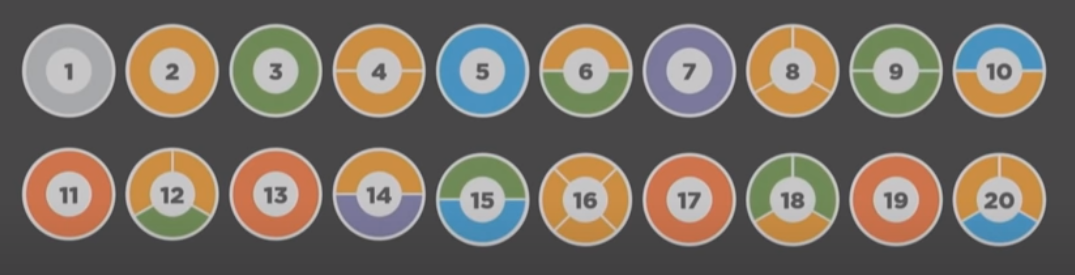
\includegraphics[width=0.5\linewidth]{numbers-and-colors.png}
    \caption{The First 20 Numbers}
    \label{fig: num-col}
\end{figure}

\Prob{
Look at Figure \ref{fig: num-col}. What do you think of the colors? Is there a pattern in which the colors appear?

How will you color numbers $21$, $22$, and $23$?
}{2}
\end{document}
